% ----
% COMP1204 CW1 Report Document
% ----
\documentclass[]{article}
\usepackage{listings}
\usepackage{xcolor}
\usepackage{sectsty}
\usepackage[margin=1in]{geometry}
\usepackage[font=small,labelfont=bf]{caption}

\usepackage{graphicx}
\graphicspath{ {./images/} }

%Change paragraphs font
\paragraphfont{\Large}

%Colors defined below
\definecolor{codegreen}{rgb}{0,0.6,0}
\definecolor{codegray}{rgb}{0.5,0.5,0.5}
\definecolor{codepurple}{rgb}{0.58,0,0.82}
\definecolor{backcolour}{rgb}{0.95,0.95,0.92}

%Code listing style
\lstdefinestyle{codestyle}{
  backgroundcolor=\color{backcolour}, commentstyle=\color{codegreen},
  keywordstyle=\color{magenta},
  numberstyle=\small\color{codegray},
  stringstyle=\color{codepurple},
  basicstyle=\ttfamily\normalsize,
  breakatwhitespace=false,
  breaklines=true,
  captionpos=b,
  keepspaces=true,
  numbers=left,
  numbersep=5pt,
  showspaces=false,
  showstringspaces=false,
  showtabs=false,
  tabsize=2
}

\lstset{style=codestyle}
\begin{document}

\title{COMP1204: Data Management \\ Coursework One: Hurricane Monitoring }
\author{Karlie Moyo \\ 32161204}
\maketitle

\section{Introduction}
This coursework covers three key topics: Unix, Latex, and Git. The coursework is divided into three parts: Unix scripting for file processing, report writing using Latex and use of Git for version control. We have been provided data about storms in KML format and were tasked with extracting the data of interest and converting it to CSV format for later processing.\\ This document details how the bash script that accomplishes the task works and shows the resulting plots of the storm data refined with the script. Also, in the process, this report aims to demonstrate the use of LaTex for report writing.

\section{Create CSV Script}
Below is the full script used to retrieve the data from KML files with comments explaining each commands purpose. The script is split in 3 main part: cleaning the data, organizing it in the correct format and exporting the result to the CSV file with the correct column headers.\\

\begin{lstlisting}[language=Bash, caption=CSV Script]
#!/bin/bash

# Getting arguments for input and output file
# Variable for regex patterns for later use delimited by '\|'
INPUT="$1"
OUTPUT="$2"
REGEX=".*UTC.*\|.*\<N\>\|.*\<S\>\|,\s.*\<W\>\|,\s.*\<E\>\|.*knots\|.*mb"

# Conversion information and starting progress bar
echo "Converting ${INPUT} -> ${OUTPUT}..."
echo -ne '[                         ] (0%)\r'
sleep 0.3

# Cleaning up the input
# cat - prints contents of file
# sed - removes the html style tags
# awk - assignment in awk removes leading and trailing spaces/tabs
# grep - prints the lines that match the regex expressions
# sed - removes the leading ', ' for West/East elements
echo -ne '[#####                    ] (33%)\r'
CLEAN=$(sed -e 's/<[^>]*>//g' ${INPUT} | awk '{$1=$1};{print}' | grep -o ${REGEX} | sed -e 's/, //g')
sleep 0.3

# Formatting the output
# echo - get the contents of the cleaned input
# sed - remove the 2 duplicate dates from every 7 line block
# tr - replaces new lines with commas
# sed - puts the new line back to create rows of 5 values of interest
echo -ne '[#############            ] (66%)\r'
RESULT=$(echo "${CLEAN}" | sed -n '3~7p;4~7p;5~7p;6~7p;7~7p' | tr "\n" "," | sed 's/,/\n/5;P;D')
sleep 0.3

# Append labels and output the result to csv
echo -ne '[#########################] (100%)\r'
APPEND=$'Timestamp,Latitude,Longitude,MinSeaLevelPressure,MaxIntensity\n'
echo "${APPEND}${RESULT}" > "${OUTPUT}"

# Stop the progress bar
echo -ne '\n'
\end{lstlisting}

\section{Storm Plots}

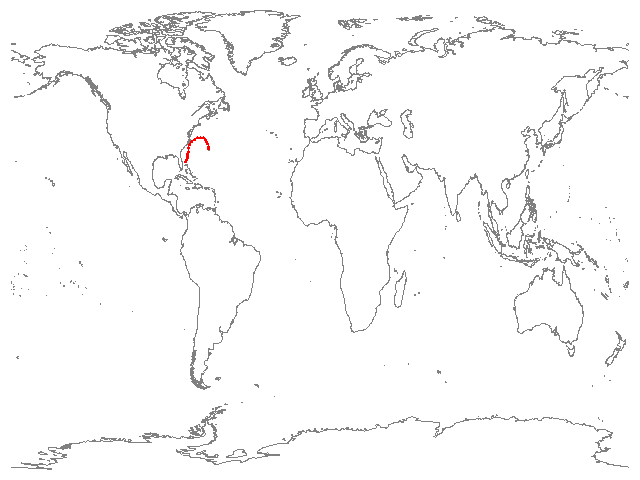
\includegraphics[width=0.8\linewidth]{storm_plot012020.png}
\captionof{figure}{Storm plot for al012020.kml}

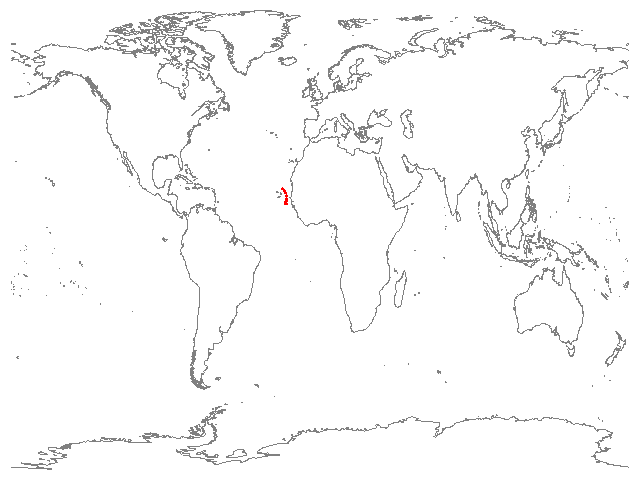
\includegraphics[width=0.8\linewidth]{storm_plot102020.png}
\captionof{figure}{Storm plot for al102020.kml}
\bigbreak \bigbreak
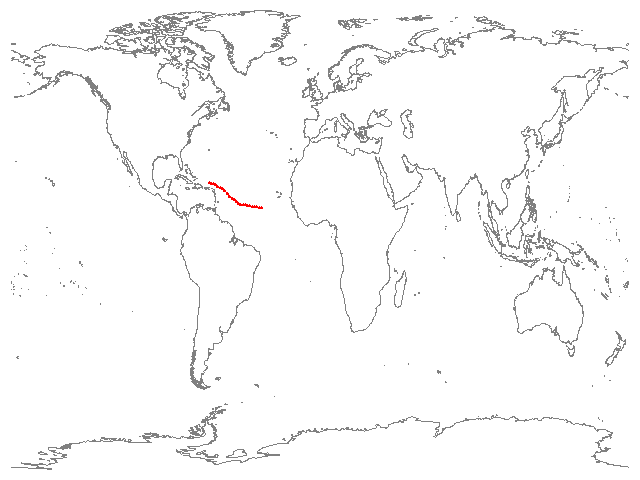
\includegraphics[width=0.8\linewidth]{storm_plot112020.png}
\captionof{figure}{Storm plot for al112020.kml}

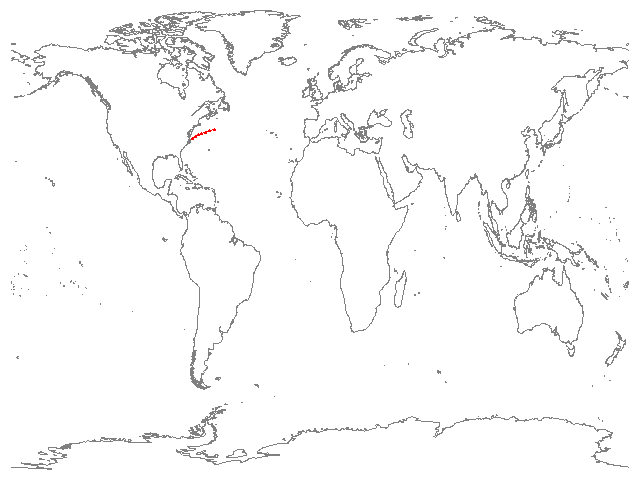
\includegraphics[width=0.8\linewidth]{storm_plot122020.png}
\captionof{figure}{Storm plot for al122020.kml}
\bigbreak \bigbreak
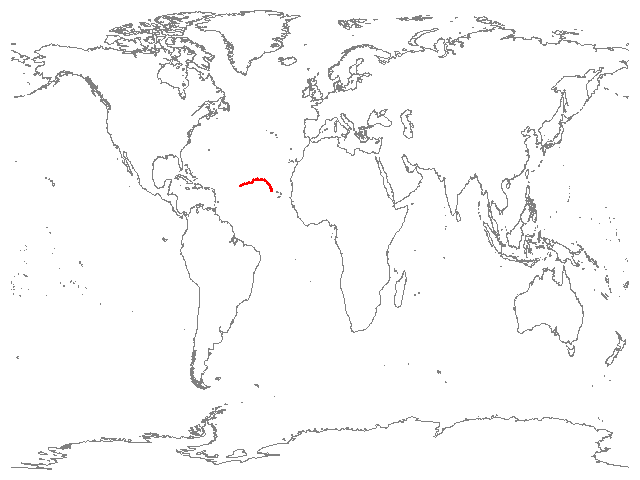
\includegraphics[width=0.8\linewidth]{storm_plot212020.png}
\captionof{figure}{Storm plot for al212020.kml}

\end{document}